\documentclass[12pt]{report} % Default font size is 11pt, it can be changed here
\usepackage[a4paper, left=3cm, right=2cm, top=3cm, bottom=2cm]{geometry} % Required to change the page size to A4
\usepackage[utf8]{inputenc} % Required for Brazilian accents - ISO-8859-1 format
\usepackage[square,authoryear]{natbib}
\usepackage[brazil]{babel} % Required for Brazilian hyphenation
\usepackage[T1]{fontenc} % Required for Brazilian hyphenation
\usepackage[brazilian,hyperpageref]{backref}
\usepackage[dvipsnames,svgnames,table,xcdraw]{xcolor}
\usepackage{amsmath}
\usepackage{booktabs}
\usepackage{colortbl}
\usepackage{datagidx}
\usepackage{fancyhdr} 
\usepackage{float} 
\usepackage{framed}
\usepackage{graphicx}
\usepackage{hyperref}
\usepackage{indentfirst}
\usepackage{makeidx}
\usepackage{multicol}
\usepackage{multirow}
\usepackage{ragged2e}
\usepackage{sectsty}
\usepackage{setspace}
\usepackage{titlesec}
\usepackage{tocloft}
\usepackage{wrapfig} 
\usepackage{xcolor}
\usepackage{mathptmx}
\usepackage{subfig}	% required for subfloats (subfigures, subtables...)
\usepackage[labelfont=bf]{caption} %Labels in bold

\usepackage{pdfpages} % requerido para incluir a página pdf com a ficha catalográfica

\usepackage{chngcntr}
\counterwithout{figure}{chapter}
\counterwithout{table}{chapter}

%Data formatada mês, ano
\usepackage[pt-BR]{datetime2}
\DTMlangsetup{showdayofmonth=false}

%\usepackage{algorithm}
\usepackage{amssymb}
\usepackage[noend]{algpseudocode}	% pseudo-codigo
\usepackage[portuguese,ruled,linesnumbered,algochapter,titlenumbered]{algorithm2e}

\makeatletter
\def\BState{\State\hskip-\ALG@thistlm}
\makeatother

%\linespread{1.5} 
\renewcommand {\baselinestretch}{1.5}

\setlength\parindent{1.25cm} 
\renewcommand{\backrefpagesname}{Citado na(s) página(s):~}

\renewcommand{\backref}{}

\definecolor{dark-red}{rgb}{0,0,0} % preto - para adequar ao modelo nortese
\definecolor{dark-blue}{rgb}{0.15,0.15,0.4}
\definecolor{medium-blue}{rgb}{0,0,0.5}
\hypersetup{
	colorlinks, linkcolor={dark-red},
	citecolor={dark-blue}, urlcolor={medium-blue}
}

% Numeracao Pagina
\pagestyle{fancy}
\fancyhf{}
\fancyheadoffset{0cm}
\renewcommand{\headrulewidth}{0pt} 
\renewcommand{\footrulewidth}{0pt}
\fancyhead[R]{\thepage}
\fancypagestyle{plain}{%
	\fancyhf{}%
	\fancyhead[R]{\thepage}%
}

%Capítulos centralizados
\chapterfont{}
\sectionfont{\normalsize \bfseries \flushleft}


% Numeracao capitulos em romano
%\renewcommand{\thechapter}{\Numeric{chapter}}
\titleformat{\chapter}[display] 
{\fontsize{18pt}{\baselineskip}\selectfont\bfseries}{\chaptertitlename\ \thechapter}{2em}{}
\titlespacing*{\chapter}{0pt}{-2em}{2em}

\titleformat{\section}[hang] 
{\fontsize{14pt}{\baselineskip}\selectfont\bfseries}{\thesection}{2em}{}
\titlespacing*{\section}{0pt}{1em}{1em}

\titleformat{\subsection}[hang] 
{\fontsize{14pt}{\baselineskip}\selectfont\bfseries}{\thesubsection}{2em}{}
\titlespacing*{\subsection}{0pt}{1em}{1em}

% centraliza Sumario
\setlength{\cftbeforetoctitleskip}{-2em}
\setlength{\cftaftertoctitleskip}{2em}
\renewcommand{\cfttoctitlefont}{\hfill\large\bfseries} 
\renewcommand{\cftaftertoctitle}{\hfill}
\addto\captionsbrazil{\renewcommand*\contentsname{\fontsize{16pt}{\baselineskip}\selectfont \textbf{SUMÁRIO}}}

% Centraliza Lista de Tabelas
\setlength{\cftbeforelottitleskip}{-2em}
\setlength{\cftafterlottitleskip}{2em}
\addto\captionsbrazil{\renewcommand*\listtablename{\fontsize{16pt}{\baselineskip}\selectfont \textbf{LISTA DE TABELAS}}}
\renewcommand{\cftlottitlefont}{\hfill\bfseries\large} 
\renewcommand{\cftafterlottitle}{\hfill}
\newlength{\mylen}
\renewcommand{\cfttabpresnum}{TABELA\enspace}
\renewcommand{\cfttabaftersnum}{:}
\settowidth{\mylen}{\cfttabpresnum\cfttabaftersnum}
\addtolength{\cfttabnumwidth}{\mylen}

% Centraliza Lista de Figuras
\setlength{\cftbeforeloftitleskip}{-2em}
\setlength{\cftafterloftitleskip}{2em}
\addto\captionsbrazil{\renewcommand*\listfigurename{\fontsize{16pt}{\baselineskip}\selectfont \textbf{LISTA DE FIGURAS}}}
\renewcommand{\cftloftitlefont}{\hfill\bfseries\large} 
\renewcommand{\cftafterloftitle}{\hfill}
\renewcommand{\cftfigpresnum}{FIGURA\enspace}
\renewcommand{\cftfigaftersnum}{:}
\settowidth{\mylen}{\cftfigpresnum\cftfigaftersnum}
\addtolength{\cftfignumwidth}{\mylen}

% Centraliza Lista de Algoritmos
\renewcommand*\listalgorithmcfname{\hfill \fontsize{16pt}{\baselineskip}\selectfont \textbf{LISTA DE ALGORITMOS} \hfill}

\newcolumntype{L}[1]{>{\raggedright\let\newline\\\arraybackslash\hspace{0pt}}m{#1}}
\newcolumntype{C}[1]{>{\centering\let\newline\\\arraybackslash\hspace{0pt}}m{#1}}
\newcolumntype{R}[1]{>{\raggedleft\let\newline\\\arraybackslash\hspace{0pt}}m{#1}}

\newcommand\Tstrut{\rule{0pt}{2.6ex}} % = `top' strut
\newcommand\Bstrut{\rule[-0.9ex]{0pt}{0pt}} % = `bottom' strut
\newcommand{\specialcell}[2][c]{%
	\begin{tabular}[#1]{@{}c@{}}#2\end{tabular}}

\graphicspath{{./figures/}}


%- COMEÇAR A EDITAR A PARTIR DESTA PARTE

\newgidx{acronym}{\hfill \fontsize{16pt}{\baselineskip}\selectfont \textbf{LISTA DE ABREVIAÇÕES} \hfill}
\newgidx{symbol}{\fontsize{16pt}{\baselineskip}\selectfont \textbf{LISTA DE SÍMBOLOS}}

\DTLgidxSetDefaultDB{acronym}
%-----------------------------------------------
% Abreviações
%-----------------------------------------------
\newacro{HTML}{\textit{HyperText Markup Language}}
\newacro{CSS}{\textit{Cascading Style Sheets}}
\newacro{GPS}{\textit{Global Positioning System}}
\newacro{APP}{\textit{Application}}
\newacro{CEFET}{Centro Federal de Educação Tecnológica Celso Suckow Da Fonseca}
\newacro{RJ}{Rio de Janeiro}

\begin{document}
	%----------------------------------------------------------------------------------------
	%	TITLE PAGE
	%----------------------------------------------------------------------------------------
	\pagenumbering{gobble}% Remove page numbers (and reset to 1)
	\pagenumbering{roman}
	%\begin{titlepage}
	
	\thispagestyle{empty} % sem numeracao
	\newgeometry{left=3cm, right=2cm, top=3cm, bottom=2cm}
	\center % Center everything on the page
	
	\begin{minipage}{\textwidth}
		\begin{center}
			{\bfseries \large CENTRO FEDERAL DE EDUCACAÇÃO TECNOLÓGICA\\ CELSO SUCKOW DA FONSECA}\\[16em]
			{\bfseries \LARGE Biblioteca Multiplataforma de Avaliação de Viagens Rodoviárias para Dispositivos Móveis}
		\end{center}
	\end{minipage}\\[6em]
	
	\begin{flushright}
		\begin{minipage}{0.5\textwidth}
			\normalsize
			\raggedleft \normalsize Luan Marcelo de Aristeu Vilarin Moraes
			\raggedleft \normalsize Thiago Della Libera Moreira
		\end{minipage}\\[6em]

	\end{flushright}
	
	\begin{flushright}
		\begin{minipage}{0.5\textwidth}
			\raggedleft
			Prof. Orientador:\\
			Renato Mauro, M.Sc.
		\end{minipage}\\
	\end{flushright}
	\vfill	
	{\bfseries \large Rio de Janeiro,\\
		\today} % Date, change the \today to a set date if you want to be precise
	
	%\end{titlepage}
	\pagebreak
	
	%----------------------------------------------------------------------------------------
	%	FOLHA DE ROSTO
	%----------------------------------------------------------------------------------------
	
	%\begin{titlepage}
	\thispagestyle{empty} % sem numeracao
	\newgeometry{left=3cm, right=2cm, top=3cm, bottom=2cm}
	\center % Center everything on the page
	
	\begin{minipage}{\textwidth}
		\begin{center}
			{\bfseries \large CENTRO FEDERAL DE EDUCACAÇÃO TECNOLÓGICA\\ CELSO SUCKOW DA FONSECA}\\[6em]
			{\bfseries \LARGE Biblioteca Multiplataforma de Avaliação de Viagens Rodoviárias para Dispositivos Móveis}\\[6em]% Title of your document
		\end{center}
	\end{minipage}\\[6em]
	
	\begin{flushright}
		\begin{minipage}{0.5\textwidth}
			\normalsize
			\raggedleft \normalsize Luan Marcelo de Aristeu Vilarin Moraes
			\raggedleft \normalsize Thiago Della Libera Moreira
		\end{minipage}\\[6em]

	\end{flushright}
	
	\begin{flushright}
		\begin{minipage}{0.5\textwidth}
			\normalsize
			\raggedleft
			Projeto final apresentado em cumprimento às normas do Departamento de Educação Superior do \acr{CEFET} no \acr{RJ}, como parte dos requisitos para obtenção do título de Bacharel em Ciência da Computação.
		\end{minipage}\\[6em]
	\end{flushright}
	
	\begin{flushright}
		\begin{minipage}{0.5\textwidth}
			\raggedleft
			Prof. Orientador: \\
			Renato Mauro, M.Sc.
		\end{minipage}\\
	\end{flushright}
	\vfill	
	{\bfseries \large Rio de Janeiro,\\
		\today} % Date, change the \today to a set date if you want to be precise
	
	%\end{titlepage}
	\pagebreak
	
	%----------------------------------------------------------------------------------------
	%	Ficha Catalografica
	%----------------------------------------------------------------------------------------
	
	%\pagenumbering{gobble}% Remove page numbers (and reset to 1)
	
	%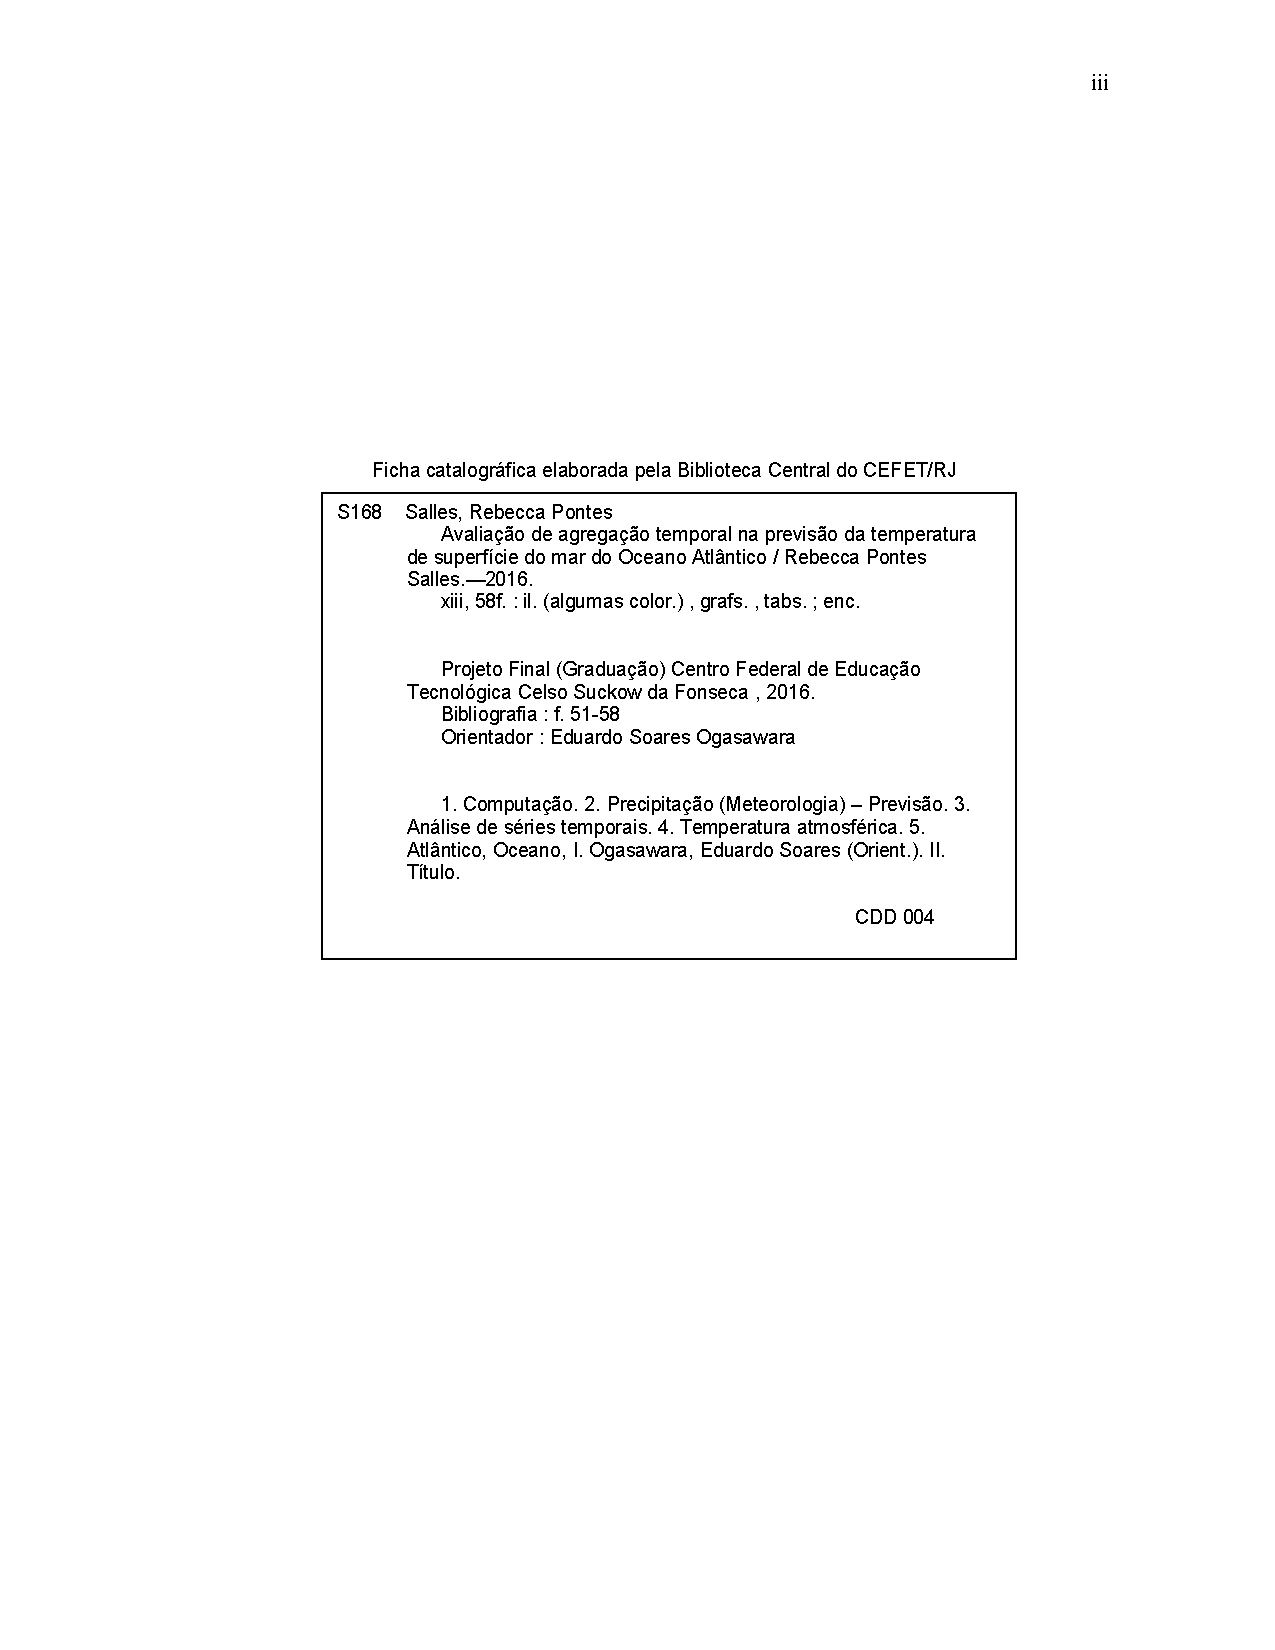
\includepdf{ficha.pdf} página pdf feita pela biblioteca
	
	\iffalse % COMENTÁRIO
	\center % Center everything on the page
	
	\fbox{%
		\hspace{1cm}
		\parbox{0.6\textwidth}{%
			\footnotesize

			Moraes, Luan Marcelo de Aristeu Vilarin; Moreira, Thiago Della Libera.
			
			\hspace{0.3cm} Biblioteca Multiplataforma de Avaliação de Viagens Rodoviárias para Dispositivos Móveis /  Luan Marcelo de Aristeu Vilarin Moraes e Thiago Della Libera Moreira. -- 2017. 

			
			\hspace{0.3cm} \pageref{lastpretextualpage},   \pageref{lastpage}f; enc.
			\singlespacing
			\hspace{0.3cm} Projeto Final (Graduação), Centro Federal de Educação Tecnológica Celso Suckow da Fonseca, 2016. 
			
			\hspace{0.3cm} Bibliografia: f, \pageref{bibpage}--\pageref{bibfinalpage}
			
			\doublespacing
			
			\hspace{0.3cm} \textit{1. Modelos de previsão 2. Séries temporais 3. Agregação temporal 4. Temperatura da superfície do mar 5. Oceano Atlântico I. Título}
		}%
	}
	\fi % FIM DO COMENTÁRIO
	
	\pagebreak
	
	%----------------------------------------------------------------------------------------
	%	Dedicatória
	%----------------------------------------------------------------------------------------
	
	{\fontsize{16pt}{\baselineskip}\selectfont \textbf{DEDICATÓRIA}}
	%\thispagestyle{empty}
	\vspace*{15em}%
	\begin{flushright}
		\begin{minipage}{0.5\textwidth}
			\raggedleft \normalsize A Deus e Google, à minha família amada que me ajudaram, apoiaram e guiaram ao longo de toda a minha vida.
		\end{minipage}\\[1.5cm]
	\end{flushright}
	
	\pagebreak
	
	%----------------------------------------------------------------------------------------
	%	Agradecimentos
	%----------------------------------------------------------------------------------------
	
	{\fontsize{16pt}{\baselineskip}\selectfont \textbf{AGRADECIMENTOS}}
	%\thispagestyle{empty}
	\vspace*{10em}%
	\begin{flushright}
		\begin{minipage}{0.5\textwidth}
			\normalsize
			Agradece-se também as contribuições de ... que deu início a pesquisas sobre o tema abordado.
		\end{minipage}\\[1.5cm]
	\end{flushright}
	
	\pagebreak
	
	%----------------------------------------------------------------------------------------
	%	Resumo
	%----------------------------------------------------------------------------------------
	
	\begin{center}
		{\fontsize{16pt}{\baselineskip}\selectfont \textbf{RESUMO}}\\[2em]
	\end{center}
	
	\justifying 
	\noindent
	A chegada da telefonia móvel às mãos da população comum permite que sensores caros e antes pouco utilizados pelas massas se tornem muito mais acessíveis. Com isso, a pesquisa focada na utilização de tais sensores também cresceu. Essa crescente mostrou a capacidade que tais dispositivos possuem quanto à coleta de dados gerais do dia-a-dia de seu dono. Porém, uma má prática foi desenvolvida em meio à essas descobertas. A grande maioria dos trabalhos envolvendo tecnologia móvel e o uso de seus sensores recria os algoritmos utilizados para coleta, limpeza, normalização e/ou apresentação dos dados. Gerando assim, uma perda de reutilização de tecnologias já criadas e já executadas, apenas por um questão de customização da aplicação. Este trabalho, oferece uma biblioteca no qual o objetivo é modularizar os passos que são recriados repetidas vezes nestes projetos oferencendo um certo grau de customização.  
	\\[3em]
	
	\normalsize\noindent
	\textbf{Palavras-chave}: aplicações híbridas, javascript, celular móvel, biblioteca, geolocalização, qualidade, direção
	
	
	Revisar RESUMO e Abstract\\
	MELHORAR INTRO\\
	ATUALIZAR ABREVIAÇÕES\\
	ATUALIZAR LISTA DE FIGURAS\\
	ATUALIZAR LISTA DE TABELAS\\
	CRIAR TABELAS DE TRABALHOS RELACIONADOS\\
	LEVANTAR ABREVIACOES\\
	MELHORAR CONCEITOS PRELIMINARES\\
	MELHORAR PROSPOSTA\\
	MELHORAR ESTADO ATUAL DO TRABALHO\\
	PLANEJAR O PLANEJAMENTO\\
	VERIFICAR REFERENCIAS\\
	FICHA BIBLIOTECA\\
	
	\pagebreak
	
	%----------------------------------------------------------------------------------------
	%	Abstract
	%----------------------------------------------------------------------------------------
	
	\begin{center}
		{\fontsize{16pt}{\baselineskip}\selectfont \textbf{ABSTRACT}}\\[2em]
	\end{center}
	
	\justifying
	\noindent
	The arrival of mobile phones in hands of population allowed expensive sensors to become much more accessible to the masses. As a result, research focused on the use of such sensors has also grown. This increase has shown the ability of such devices to collect their users day-to-day data important to learn, correct and enhance daily activities. However, a bad practice was developed in the midst of these findings. The vast majority of the work involving mobile technology and the use of its sensors recreates the algorithms used for data collection, cleaning, normalization and/or presentation. Generating, thus, a loss of reuse of technologies already created and already executed, just for the sake of customization of the application. This work offers a library in which the objective is to modularize the steps that are recreated repeatedly in these projects offering a certain degree of customization.
	\\[3em]
	
	\normalsize\noindent
	\textbf{Keywords}: hybrid applications, javascript, mobile phone, library, gps, quality, driving
	
	
	\pagebreak
	
	%----------------------------------------------------------------------------------------
	%	TABLE OF CONTENTS
	%----------------------------------------------------------------------------------------
	
	\renewcommand{\cftdot}{}
	\tableofcontents % Include a table of contents 
	
	\pagebreak
	
	%----------------------------------------------------------------------------------------
	%	TABLE OF FIGURES
	%----------------------------------------------------------------------------------------
	
	\listoffigures
	
	\pagebreak
	
	%----------------------------------------------------------------------------------------
	%	TABLE OF TABLES
	%----------------------------------------------------------------------------------------
	
	\listoftables
		
	\pagebreak
	
	%----------------------------------------------------------------------------------------
	%	Lista de Abreviações
	%----------------------------------------------------------------------------------------
	
	\printterms[database=acronym,columns=1,prelocation=hfill,style=align]
	
	\label{lastpretextualpage}
	\pagebreak
	
	
	\pagenumbering{arabic}
	\justifying
	
\chapter{Introdução}
\label{sec:introducao}

Diversos trabalhos propõem-se a coletar e interpretar informações de modo a identificar padrões que respondam questionamentos acerca da qualidade do serviço de transporte multimodal em várias localidades do planeta. Inúmeros fatores podem vir a influenciar o conforto da viagem e o grau de satisfação do passageiro para com a experiência entregue pela companhia de transporte. 

Algumas características podem porém gerar danos à segurança dos passageiros. \citep{world2015global} aponta a relação entre a condição da malha viária e o índice de acidentes fatais no trânsito. \citep{euPolicyDep} afirma que o comportamento do motorista é, juntamente com a qualidade da infraestrutura disponível, o maior contribuidor para que acidentes aconteçam. Logo, é possível achar uma justificativa plausível para que tantos trabalhos tentem identificar padrões nas viagens afim de tentar mitigar algumas das situações apontadas como possíveis causas de acidentes.

\chapter{Conceitos Preliminares}
\label{sec:conceitos_preliminares}

\section{Aplicações Híbridas}
Hoje o total de aplicações para celulares (\acr{APP}s), nas diversas lojas de aplicativos existentes, somam o montante maior do que o de dois milhões \cite{malavolta} de aplicativos disponíveis. Relatórios passados do Gartner \cite{gartner} previam que o volume de downloads de aplicações para celulares ultrapassaria trezentos bilhões em 2016. Isso deixa claro que as aplicações para dispositivos móveis têm sua posição já consolidada dentro da sociedade.

Com isso algumas dificuldades também ficam aparentes. O processo de desenvolvimento de aplicações nativas, apesar de ser a maneira mais apropriada de criar-se uma aplicação para celulares, apresenta algumas desvantagens \cite{Xanthopoulos:2013:CAC:2490257.2490292}. A maior delas é provavelmente o fato de não ser possível reutilizar o código de uma aplicação entre plataformas de desenvolvimento (sistema operacional) diferentes. Com isso, e por sua maior complexidade de desenvolvimento, aplicações nativas requerem uma maior e mais experiente equipe de desenvolvimento.

Como uma possível solução para o problema supracitado, usa-se a abordagem de desenvolvimento de uma aplicação híbrida. Uma aplicação híbrida é uma ramificação das soluções ditas multiplataforma (\textit{cross-platform}), como: \textit{Web \acr{APP}s}, \textit{Hybrid \acr{APP}s}, \textit{Interpreted Apps} e \textit{Generated \acr{APP}s} \cite{Xanthopoulos:2013:CAC:2490257.2490292}. Resumidamente, aplicações híbridas são \textit{aplicações web} dentro de um invólucro de aplicação nativa \cite{Serrano:2013:MWA:2553372.2553378}, a aplicação tem o código de suas telas salvos fisicamente no aparelho porém utiliza uma \textit{webview} para mostrá-las. 

Tais aplicações são desenvolvidas utilizando tecnologias como \acr{HTML}, \acr{CSS} e JavaScript, diminuindo consideravelmente a curva de aprendizado de um desenvolvedor para que o mesmo seja capaz de criar uma aplicação para dispositivos móveis. Faz-se uso também de um \textit{framework} híbrido de desenvolvimento \textit{e.g.} Apache Cordova, Ionic Framework, ou React Native. Esses frameworks são responsáveis por encapsular a aplicação em uma interface nativa, dando inclusive acesso à interface de interação com ferramentas do sistema.

As vantagens de criar-se uma aplicação dessas é justamente a capacidade de escrever seu código apenas uma vez e mesmo assim o aplicativo poderá ser usado em diferentes ambientes, é o chamado \textit{write once, run anywhere} \cite{Xanthopoulos:2013:CAC:2490257.2490292}. Além dessa vantagem óbvia, por usar JavaScript, desenvolvedores podem lançar mão facilmente da grande comunidade da linguagem e reutilizar inúmeras bibliotecas voltadas para \textit{web} em suas aplicações.

Já suas principais desvantagens estão no desempenho ao acessar a interface do sistema \cite{malavolta}, pois é preciso utilizar códigos intermediários para traduzir o que a aplicação em JavaScript deseja para com o acesso do sistema, e o desempenho e fluídez na transição de telas, haja vista que são renderizadas como dentro de um navegador.


\chapter{Trabalhos Relacionados}
\label{sec:trabalhos_relacionados}

Utilizando-se de estratégias menos complexas ou mais robustas, inúmeros são os trabalhos dedicados ao levantamento e processamento de informações para entender e melhorar a infraestrutura das estradas ou o comportamento do motorista no trânsito. \citep{gawad2016dynamic} propõem uma abordagem de detecção de anomalias na pista utilizando aprendizado de máquina para calcular o limite entre um balanço natural do automóvel e um buraco no asfalto. Seu trabalho é dividido entre a aplicação em um telefone móvel, utilizada para perceber anomalias e apresentar um mapa com as marcações de outros eventos levantados anteriormente por mais usuários. E, um servidor que utiliza aprendizado por reforço para inserir ou remover anomalias no banco de dados. 

\citep{HANAOKA2014274} estuda a aplicabilidade de interpretar dados sobre o trajeto diário de estudantes da Universidade de Ritsumeikan em Kyoto, Japão. Em seu trabalho, os autores estimam as rotas dos estudantes interpolando dados de serviços multimodais de transporte que representam a origem e o destino dos estudantes em horários restritos do dia. Utilizando esta abordagem tenta-se prever o deslocamento de estudantes e a área de maior concentração dos mesmos na respectiva fatia temporal diária. Podendo assim o trafego ao redor da universidade e a oferta de transporte até a mesma serem melhor estruturados.

Em \citep{kim2009passenger} apresenta-se uma modelagem a partir de uma entrevista em forma de questionário que visa predizer o comportamento de passageiros baseado na probabilidade de escolha entre o primeiro ônibus a chegar à parada e o segundo. Tendo como características determinante o conforto da viagem baseado na disponibilidade de assentos, lotação do veículo e o tempo de duração do trajeto.

Já \citep{raymond2016} debruça-se sobre a questão da difícil interpretação de séries-temporais advindas do sistema \acr{GPS}, já que as mesmas podem vir a apresentar \textit{outliers} cuja origem é a interferência que o sinal de geolocalização pode vir a receber. Para evitar tratar tal desafio é utilizado uma técnica de correspondência por mapas (\textit{map-matching}) e \textit{bag of words}, esta última sendo uma técnica de classificação de imagem. A correspondência por mapas transforma uma sequência de pontos do \acr{GPS} em uma de ruas, diminuindo a granularidade do problema. Para testar tal abordagem é utilizado a base de dados de posições dos ônibus da cidade do Rio de Janeiro. 

\cite{SINGH201756} FALAR DO LIVRO DE 30 pags


\begin{table}[!ht]
	\centering
	\caption{Comparação dos trabalhos relacionados}
	\begin{tabular}{ L{6cm} C{1.5cm} C{1.5cm} C{1.5cm} C{1.5cm} }
		\hline\noalign{\smallskip}
		Trabalho & Original & Framework & Entrevista \\
		\hline\noalign{\smallskip}
		%\hline\noalign{\smallskip}
		\citet{ferreira2013visual} & X &  &  & \\
		\citet{andrienko2008spatio} & X &  &  & \\
		\citet{adrienko2011spatial} &  & X &  & \\
		\citet{cassisi2013motif} &  &  & X & \\
		\citet{jiang2008finding} &  &  & X & \\
		\citet{chi2012face} &  &  & X & \\
		\citet{schneider2013unravelling} &  &  &  & X \\
		\hline\noalign{\smallskip}
	\end{tabular}
	\label{tbl:sumario}
\end{table}

A tabela \ref{tbl:sumario} apresenta os trabalhos relacionados e as técnicas aplicadas. Áreas mais exploradas são a identificação de \emph{motifs} em séries temporais e a agregação espaço-temporal baseada em região. Não foram observados trabalhos associados a identificação de \emph{motifs} em séries espaço-temporais associadas a objetos permanentes. Observa-se, portanto, uma lacuna para estudo com amplo potencial de exploração.

\chapter{Proposta} 
\label{sec:proposta}

Este trabalho tem como objetivo facilitar o desenvolvimento de aplicações de coletas de dados gerais através dos sensores de um smartphone convencional ao avaliar a qualidade de direção mas não restringido apenas a esse proposito. Como citado na seção de trabalhos relacionados, a grande maioria dos trabalhos partia de um ponto inicial onde não havia nenhuma ferramenta que auxiliasse ou facilitasse a execução da pesquisa. Todos os trabalhos coletavam dados crus e trabalhavam em cima dos mesmo com, em certos casos filtros e çalculos para normalizarem os dados e assim, poder fazer uma análise dos mesmos. Mesmo tendo esse conceito em mente, a proposta de um framwork é muito mais ampla que atacar somente esse tipo de usuário. Existem possibilidades de que este framework seja utiliado no mercado por sua fácil customização e sua modularização.

A criação de um framework tem o objetivo de generalizar e facilitar a execução de qualquer tarefa sem que a mesma seja retrabalhada, seja em metodologia ou desenvolvimento, com certo grau de customização.(um objetivo). Estão sendo considerados trabalhos nos quais o objetivo é coetar e interpretar dados dos sensores do celular como acelerometro, \acr{GPS}, sensor de gravidade, giroscópio(nem sei se existe, inventei). Como a extensão do uso de um framework é muito ampla, o escopo será reduzido para atender necessidades voltadas ao processamento e avaliação da qualidade e perfil de direção de motoristas em geral.Ainda assim podemos extrai um grande quantidade de possibilidades em relação a que tipo de motorista será o alvo do trabalho. Portanto, ao final deste trabalho será apresentado uma aplicação exemplo que irá coletar dados sobre o delsocamento dos alunos do \acr{CEFET} e avaliar se a qualidade dos meios de transporte utilizados é satisfatória. 

esta avaliação é feita desta forma (elaborar isso conforme o trabalho é desenvolvido mas aqui seria interessante falar do \acr{APP} exemplo no qual o framework irá atuar)

\chapter{Estado Atual do Trabalho}
\label{sec:estado_atual}

Como descrito na seção anterior, o objetivo será elaborado um framework compilando funcionalidades de coleta de dados sensoriais. No momento, uma análise dos estudos de caso mais comuns foi feita, assim como quais funcionalidades, sensores e algoritmos seriam de grande importância como parte do framework e qual o melhor desenho de arquitetura para melhor atender as necessidades dos usuários. O desenvolvimento da tarefa segue o cronograma abaixo: (montar cronograma)

\begin{figure}[!ht]
	\centering
	\begin{minipage}[t]{0.49\textwidth}
		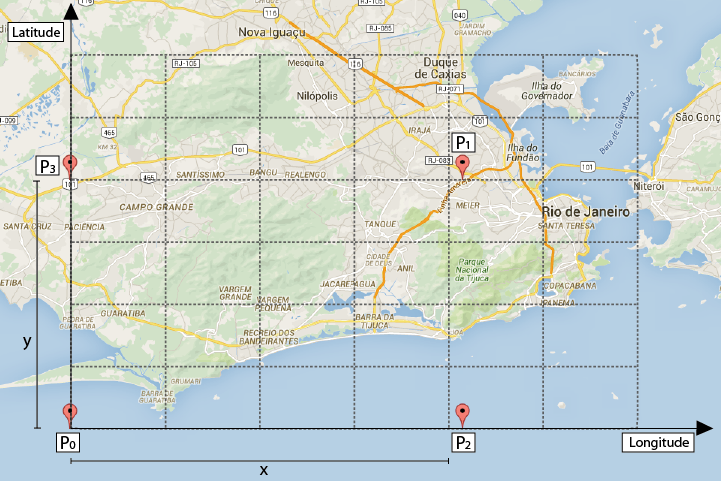
\includegraphics[width=\textwidth]{conversao.png}
		\caption
		{
			Conversão dos dados de localização dos pontos de ônibus.
		}
		\label{fig:conversao}
	\end{minipage}
	\hfill
	\begin{minipage}[t]{0.47\textwidth}
		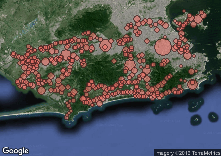
\includegraphics[width=\textwidth]{stations-v3.png}
		\caption
		{
			Estações obtidas aplicando o algoritmo de agrupamento DBSCAN sobre os pontos de ônibus do Rio de Janeiro.
		}
		\label{fig:stacoes}
	\end{minipage}	
\end{figure}

Após definir a arquitetura e casos de uso cobertos, será iniciada a implementação do framework conforme a documentação definida. O desenvolvimento será feito em Javascript e o alvo da ferramenta será aplicativos híbridos para obtermos um alcance maior(apesar de eu apenas ter visto em \acr{APP}s nativos) de usuários e sistemas operacionais.  

Concomitante ao desenvolvimento, uma documentação para o usuário será escrita com tutoriais(talvez) e exemplos de como utilizar as funcionalidades do framework. 

O conceito por trás das funcinonalidades é torna-lás o mais customizável possível para que o usuário tenha total liberdade de adicionar ou retirar funcionalidades que sejam (des)necessárias ao desenvolvimento de seu projeto. 

Para exemplificar e mostrar o poder e simplicidade por trás do framework desenvolvido. Será também desenvolvido uma aplicação simples como exemplo. Além de servir como guia para utilização do framework. Aplicativos híbridos tem um problema que é amplamente conhecido, sua perda de desempenho principalmente se o \acr{APP} for muito baseado em visualização gráfica. para contornar isso, será desenvolvido servidor simples que tratará do processamento crowdsorcing e outros tipos de processamento envolvidos. Para a comunicação com o Servidor será criado uma API que al'me de se comunicar, permitirá a contabilização de dados trocados entre o usuário e o servidor. Permitindo assim, criar uma interface de gamificação para bonificar o usuário pela coleta de dados importante para a análise de dados e uma possível forma de monetizar este trabalho através de requisições à API.

A dissertação será escrita conforme as partes que compoem a ferramentas forem desenvolvidas. Assim, é garantiremos que o conteúdo da dissertação corresponde com o trabalho feito e as demais funcionalidades citadas aqui que não forem desenvolvidas serão novamente citadas levando em consideração os impedimentos e dificuldades encontradas até o momento da defesa.

A defesa da dissertação (9:Defesa) está prevista para junho de 2018. O cronograma, indicado na tabela \ref{tbl:cronograma}, prevê as etapas abordadas neste trabalho. A tabela indica os meses de previsão de conclusão de cada uma das etapas.

\begin{table}[!ht]
	\centering
	\caption{Cronograma de desenvolvimento da dissertação}
	\begin{tabular}{ L{3cm} C{1cm} C{1cm} C{1cm} C{1cm} C{1cm} C{1cm} C{1cm} C{1cm} C{1cm} }
		\hline\noalign{\smallskip}
		Atividade & jun-jul  & ago-set & out-nov & dez-jan & fev-mar & abr-mai & jun-jul & ago-set \\
		\hline\noalign{\smallskip}
		1:Estações & X & & & & & & & \\
		2:Agr.Temp. & X & X & & & & & & \\
		3:Id.Motifs & & & X & X & & & & \\
		4:Aval.Exp. & & & & X & & & & \\
		5:Ana.Result. & & & & & X & X & & \\
		6:Fund.Teo.& X & X & & & & & & \\
		7:Metodologia & & X & X & X & & & & \\
		8:Artigo & & & & & X & X & X & \\
		9:Defesa & & & & & & & & X \\
		\hline\noalign{\smallskip}
	\end{tabular}
	\label{tbl:cronograma}
\end{table}

\label{bibpage}
\addcontentsline{toc}{section}{Referências Bibliográficas}
\bibliography{references}
\bibliographystyle{plain}
\label{bibfinalpage}


\label{lastpage}\end{document}
